\documentclass[../../main.tex]{subfiles}
\begin{document}

{\large
\textcolor{blue}{Jaime: Isto ainda é um copy paste rudimentar da minha dissertaçao,
vou ainda adaptar para o nosso paper.}\par
}

%The staggered quantum walk (SQW) model aims to spread a transition probability
%to neighboring vertices with discrete time steps. The notion of adjacency comes
%from cliques, and the initial stage of this walk consists of partitioning the
%graph into several different cliques. This is known as the \textit{tessellation} process. An
%element of a tessellation $\mathscr{T}$ is called a polygon, and it is only
%valid if all of its vertices belong to the clique in $\mathscr{T}$. The set of
%polygons of each tessellation must cover all vertices of the graph, and the set
%of tessellations $\{\mathscr{T}_{1}$,$\mathscr{T}_{2}$,...,$\mathscr{T}_{k}\}$
%must cover all the edges.\par 


The staggered quantum walk (SQW) model disperses transition probabilities
across neighboring vertices in discrete time steps, leveraging the concept of
adjacency through cliques. Initially, the graph is partitioned into cliques in
a process called \textit{tessellation}. In tessellation $\mathscr{T}$, an
element is termed a polygon if its vertices are in the same $\mathscr{T}$'s
clique. These polygons must collectively encompass all graph vertices, while
the tessellation set $\{\mathscr{T}_{1}, \mathscr{T}_{2},...,
\mathscr{T}_{k}\}$ should cover all edges.

%\footnote{A clique is defined as the subset of vertices of an undirected graph
%such that every two distinct vertices in each clique are adjacent.},

Operators $H_1,H_2,...,H_k$ are constructed to propagate probability amplitudes
locally within each polygon. The state for each polygon in the $k^{th}$
tessellation is represented as:

\begin{equation}
	\ket{u_{j}^{k}} = \frac{1}{\sqrt{|\alpha_{j}^{k}|}}\sum_{l\in\alpha_{j}^{k}}\ket{l},
\end{equation}

where $\alpha_{j}^{k}$ denotes the $j^{th}$ polygon. Associated with each
tessellation is a unitary, local, and Hermitian operator $H_k$, defined in
\cite{PhysRevA.95.012328} as

\begin{equation}
	H_k = 2\sum_{j=1}^{p}\ket{u_{j}^{k}}\bra{u_{j}^{k}} - I,
\end{equation}

The evolution operator, solving the
time-independent Schrödinger equation for $H_k$, is given by

\begin{equation}
	U = e^{i\theta_{k}H_{k}}\cdots e^{i\theta_{1}H_{1}},
\end{equation}

where each term $e^{i\theta_{k}H_{k}}$ simplifies to $\cos(\theta_k)I +
i\sin(\theta_k)H_k$, leveraging $H_k^2 = I$. This highlights $H_k$ as a
reflection operator, enabling local operation through Taylor series expansion.

%These definitions allow the construction of operators $H_1$,$H_2$,...,$H_k$ to
%propagate the probability amplitude locally, in each polygon. The state
%associated to each polygon is
%\begin{equation}
%	\ket{u_{j}^{k}} = \frac{1}{\sqrt{\mathopen|\alpha_{j}^{k}}\mathclose|}\sum_{l\in\alpha_{j}^{k}}\ket{l},
%\end{equation}
%where $\alpha_{j}^{k}$ is the $j^{th}$ polygon in the $k^{th}$ tessellation.\par
%
%The unitary, local and Hermitian operator $H_k$, associated to each tessellation is
%defined in \cite{portugal2017b} as
%\begin{equation}
%	H_k = 2\sum_{j=1}^{p}\ket{u_{j}^{k}}\bra{u_{j}^{k}} - I.
%	\label{eq:StagHamil}
%\end{equation}
%Solving the time-independent Schrodinger equation for this Hamiltonian gives
%the evolution operator 
%\begin{equation}
%	U = e^{i\theta_{k}H_{k}}...e^{i\theta_{2}H_{2}}e^{i\theta_{1}H_{1}},
%	\label{eq:stagWalkUnmodOp}
%\end{equation}
%where
%\begin{equation}
%	e^{i\theta_{k}H_{k}} = \cos{(\theta_k)}I + i\sin{(\theta_k)}H_k,
%\end{equation}
%since $H_k^2 = I$, meaning that the Hamiltonian is a reflection operator that,
%when expanded in a Taylor series, generates a local operator.\par

\subsection{SQW on the line}

The simplest use case of this quantum walk model is the one-dimensional
lattice, where the minimum tessellations are
\begin{equation}
	\mathscr{T}_{\alpha}= \{\{2x,2x+1\}\colon x \in \mathbb{Z}\},
\end{equation}
\begin{equation}
	\mathscr{T}_{\beta}= \{\{2x+1,2x+2\}\colon x \in \mathbb{Z}\}.
\end{equation}
\begin{figure}[!h]
	\centering
	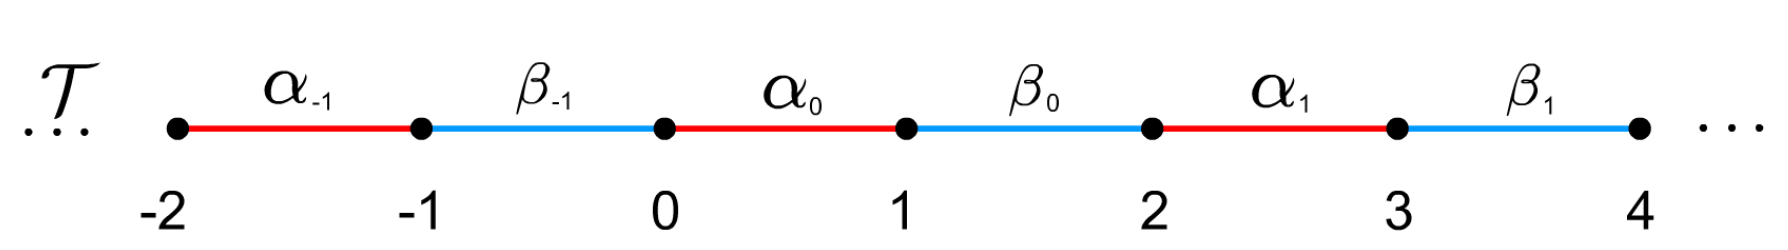
\includegraphics[scale=0.40]{img/Sec2/tesselation.png}
	\caption{Tessellation of a line graph.} 
	\label{fig:stagQWTesselation}
\end{figure}
Each element of the tessellation has a corresponding state, as can be seen in
figure \ref{fig:stagQWTesselation}, and the uniform superposition of these
states is
\begin{equation}
	\ket{\alpha_x} = \frac{\ket{2x} + \ket{2x+1}}{\sqrt{2}},
\end{equation}
\begin{equation}
	\ket{\beta_x} = \frac{\ket{2x+1}+\ket{2x+2}}{\sqrt{2}}.
\end{equation}
We can now define Hamiltonians $H_\alpha$ and $H_\beta$ as 
\begin{equation}
	H_\alpha = 2\sum_{x=-\infty}^{+\infty}\ket{\alpha_{x}}\bra{\alpha_x} - I,
	\label{eq:stagSimulHalpha}
\end{equation}
\begin{equation}
	H_\beta = 2\sum_{x=-\infty}^{+\infty}\ket{\beta_{x}}\bra{\beta_x} - I.
	\label{eq:stagSimulHbeta}
\end{equation}

The Hamiltonian evolution operator reduces to
\begin{equation}
	U = e^{i\theta H_\beta}e^{i\theta H_\alpha},
	\label{eq:stagSimulUniOp}
\end{equation}
and applying it to an initial condition $\ket{\psi(0)}$ results in the time
evolution operator
\begin{equation}
	U\ket{\psi(t)} = U^t\ket{\psi(0)}.
\end{equation}\par

Defining the time evolution operator allows for the coding of the quantum walk
with specific initial conditions and a chosen $\theta$ value, to observe the
spread of the probability distribution over time. The quantum walk's outcomes,
as depicted in figure \ref{fig:stagQW2InitCond}, reveal that starting with
$\ket{\psi(0)}=\ket{0}$ or $\ket{\psi(0)}=\ket{1}$ produces asymmetric
probability distributions. Specifically, the former initial condition favors a
peak on the left side, whereas the latter results in a peak on the right side.

\begin{figure}[!h]
	\begin{subfigure}[h]{0.50\textwidth}
	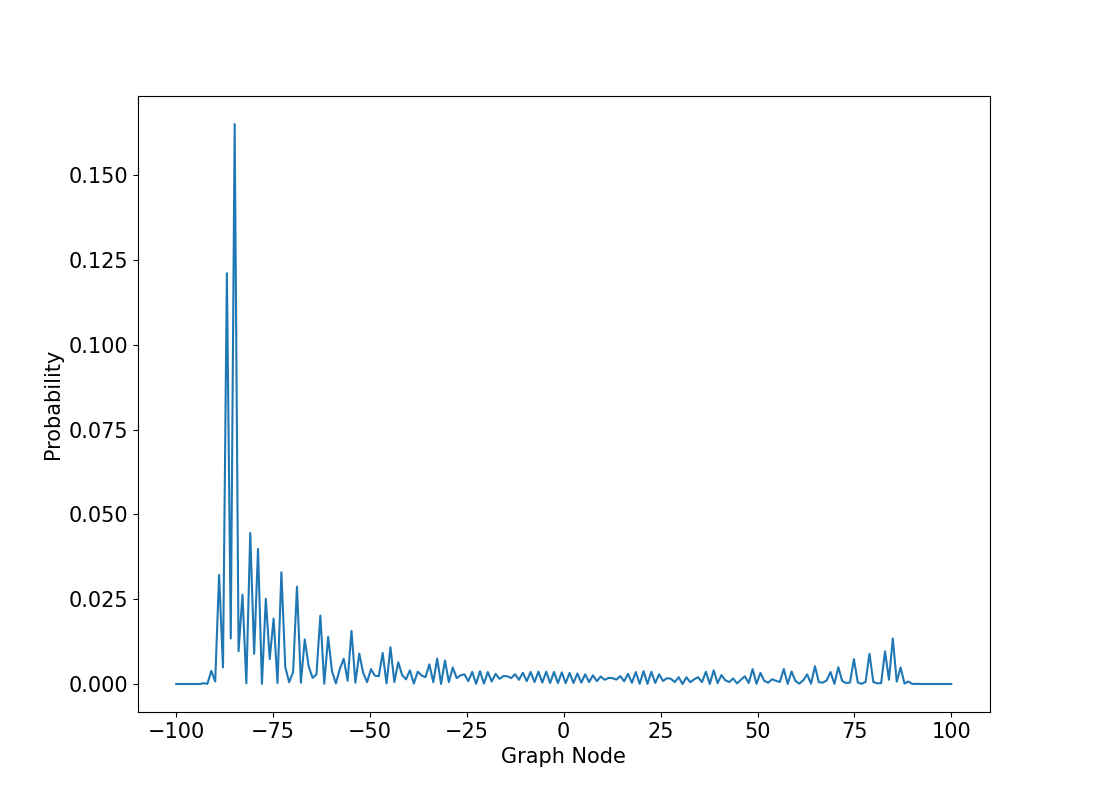
\includegraphics[width=\linewidth]{img/Sec2/stagqwSingle0.png}
	\caption{$\ket{\psi(0)}=\ket{0}$}\label{fig:fig6}
	\end{subfigure}\hfill
	\begin{subfigure}[h]{0.50\textwidth}
	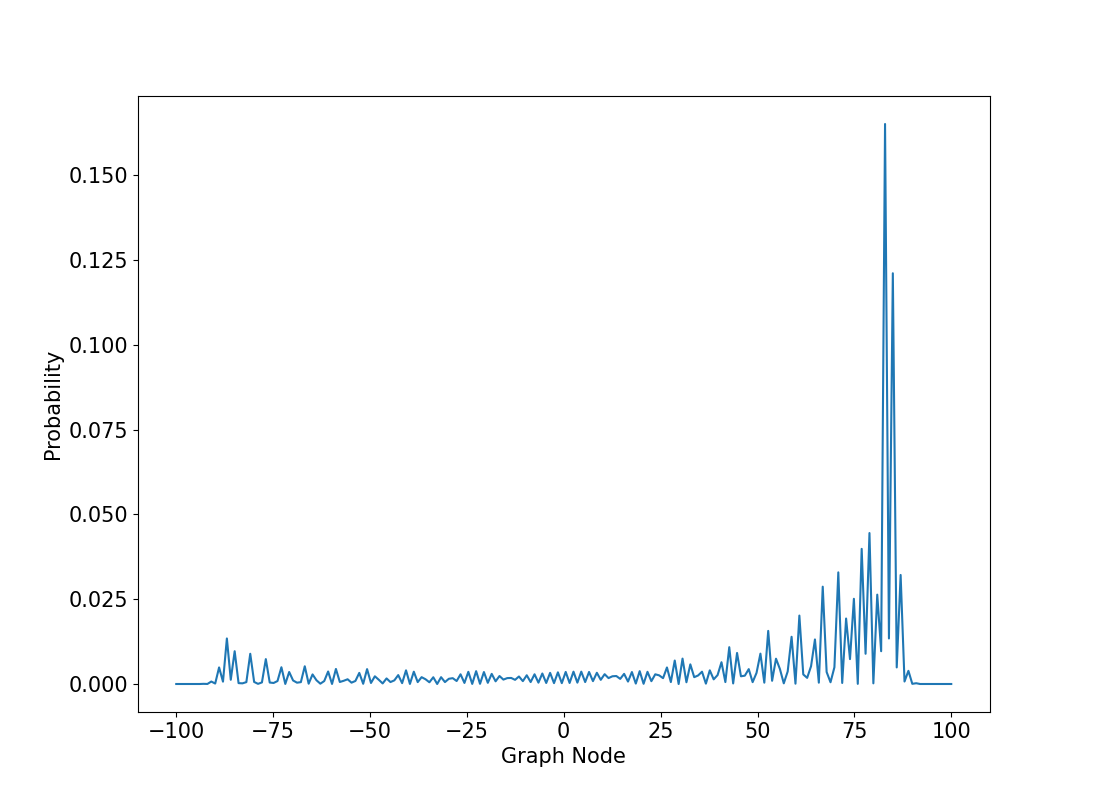
\includegraphics[width=\linewidth]{img/Sec2/stagqwSingle1.png}
	\caption{$\ket{\psi(0)}=\ket{1}$}\label{fig:fig7}
	\end{subfigure}\hfill
    \caption{Probability distributions for the staggered quantum walk on a line
    after 50 steps, for different initial conditions.}
    \label{fig:stagQW2InitCond}
\end{figure}\par

%Having defined the time evolution operator, the walk is ready to be coded with
%a certain initial condition and $\theta$ value, to better understand how the
%probability distribution spreads through time. 
%For the first case study, the initial condition will be a uniform superposition
%of states $\ket{0}$ and $\ket{1}$ and the value of $\theta$ will be varied in
%order to understand how this parameter impacts the walk, as seen in
%figure \ref{fig:stagQWSimulMultTheta}. The overall structure of the probability
%distribution is very similar for different values of $\theta$, the difference
%being that the walker is more likely to be found further away from the origin
%as the angle increases.
%

When the initial condition is a uniform superposition of $\ket{0}$ and
$\ket{1}$, varying $\theta$ helps explore its effect on the quantum walk, as
illustrated in figure \ref{fig:stagQWSimulMultTheta}. Although the probability
distribution's general structure remains consistent across different $\theta$
values, the likelihood of the walker being farther from the origin increases
with the angle.

%Another interesting case arises when the initial condition is a uniform superposition
%of states $\ket{0}$ and $\ket{1}$. Here, we vary the value of $\theta$ in
%order to understand how this parameter impacts the walk, as seen in
%figure \ref{fig:stagQWSimulMultTheta}. The overall structure of the probability
%distribution is very similar for different values of $\theta$, the difference
%being that the walker is more likely to be found further away from the origin
%as the angle increases.

\begin{figure}[!h]
	\centering
	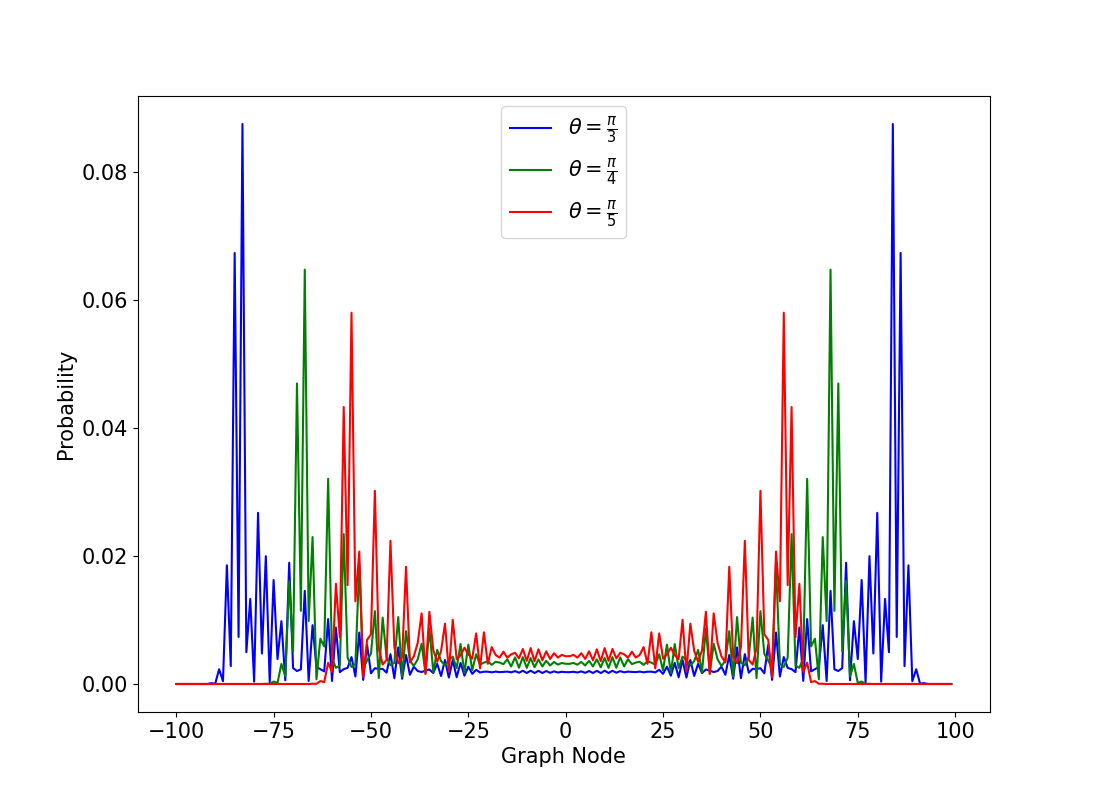
\includegraphics[scale=0.40]{img/Sec2/stagqwMultiple.png}
    \caption{Probability distribution for the staggered quantum walk on a line
    after 50 steps, with initial condition
    $\ket{\psi(0)}=\frac{\ket{0}+\ket{1}}{\sqrt{2}}$, for multiple values of
    $\theta$.} \label{fig:stagQWSimulMultTheta}
\end{figure}\par


%Another interesting case study is to see how the initial condition affects the
%dynamics of the system, and figure \ref{fig:stagQW2InitCond} shows the results
%of plotting the quantum walk for initial conditions  $\ket{\psi(0)}=\ket{0}$
%and $\ket{\psi(0)}=\ket{1}$.  Similarly to the coined case, each initial
%condition results in asymmetric probability distributions,
%$\ket{\psi(0)}=\ket{0}$ leads to a peak  in the left-hand side, while condition
%$\ket{\psi(0)}=\ket{1}$ results in a peak in the right-hand side. As shown
%in figure \ref{fig:stagQWSimulMultTheta}, the uniform superposition of both
%these conditions results in a symmetric probability distribution.\par


\subsection{Noisy Staggered Quantum Walk Model}

\begin{equation}
    U = \prod_{j} U_j(T_j(t), \theta_j(t))
\end{equation}
% \pagebreak

\end{document}
